\documentclass{beamer}

%%% -------------- CREATE HANDOUTS -----------------------------------
%\documentclass[12pt, handout]{beamer}
%\usepackage{pgfpages}
%\pgfpagesuselayout{4 on 1}[letterpaper, landscape, border shrink=5mm]
%%% ------------------------------------------------------------------


\mode<presentation>
  \usepackage{ru}
  %\usetheme{Warsaw}
  %\usecolortheme{seahorse}
  %\usefonttheme{default}
  \setbeamertemplate{caption}[numbered]
  %\setbeamertemplate{navigation symbols}{}
  \setbeamertemplate{bibliography item}[text]
\newcommand*\oldmacro{}%
	\let\oldmacro\insertshorttitle%
%\renewcommand*\insertshorttitle{%
%   \oldmacro\hfill%
%   \insertframenumber\,/\,\inserttotalframenumber}
\setbeamertemplate{section page}{
    \begin{centering}
    \vspace{1cm}
    \begin{beamercolorbox}[rounded=true,shadow=false,sep=4pt,center]{part title}
    \usebeamerfont{section title}\LARGE{\insertsection}\par
    \end{beamercolorbox}
    \end{centering}}
\usepackage{ragged2e}
\usepackage[english]{babel}
\usepackage[utf8]{inputenc}
\usepackage{appendixnumberbeamer}
\usepackage{natbib}
\usepackage{textpos}
\usepackage{lipsum}
\usepackage{tikz}
\usepackage[percent]{overpic}
\usepackage{textcomp}
\usepackage{booktabs}
\usepackage{pxfonts}
%\setbeameroption{show notes}
%\setbeamertemplate{note page}[plain]

%Change Bullets in latex list
%\renewcommand\labelitemi{$\blacktriangleright$}
%\renewcommand\labelitemii{$\coAsterisk$}

%\setbeamertemplate{background}{\tikz[overlay, remember picture]\node[xshift=-2.3cm, yshift=1.50cm, opacity=0.4]at (current page.south east){
\includegraphics[width=4cm]{images}};}

\title[Decontamination Factors for Nuclear Forensics]{Characterizaiton of Pu Separation by PUREX}
\author{Paul Mendoza}
\date{September 28, 2016}

\begin{document}
\begin{frame}
	%% background
  \tikz[overlay, remember picture]\node[xshift=-3.5cm, yshift=3cm, opacity=0.1]at (current page.south east){
\includegraphics[width=8cm]{tamu_system_proposed_seal_042915}};
	%% Left-hand logo
  \begin{tikzpicture}[remember picture, overlay]
  \node [xshift = 3 cm, yshift=1.2cm] at (current page.south west){
\includegraphics[width=5cm]{tees_logo_primary_maroon}};
  \end{tikzpicture}
    %% Right-hand logo
  \begin{tikzpicture}[remember picture, overlay]
  \node [xshift = -3cm, yshift=1.2cm] at (current page.south east){
\includegraphics[width=5cm]{TEES_NSSPI_logo_HMaroon}};
  \end{tikzpicture}
  \titlepage
\end{frame}

%Add Biola Seal
\setbeamertemplate{background}{\tikz[overlay, remember picture]\node[xshift=-2.5cm, yshift=2.5cm, opacity=0.05]at (current page.south east){
\includegraphics[width=6cm]{imageedit_2_7317234434}};}

%Add NSSPI to upper right
\addtobeamertemplate{frametitle}{}{%
  \begin{tikzpicture}[remember picture,overlay]
    \node[anchor=north east,yshift=2pt] at (current page.north east) {
\includegraphics[height=0.8cm]{TEES_NSSPI_Acronym_logo_WHT}};
    \end{tikzpicture}}



\begin{frame}{Outline}
\tableofcontents
\end{frame}

\section{Motivation}
\begin{frame}{Motivation}
\begin{itemize}
\item{Pu isotopes produced in irradiated fuel can vary depending on}
  \begin{itemize}
  \item{Burnup (irradiation history)}
  \item{Reactor neutron spectrum (core design)}
  \end{itemize}
\item{Weapons-grade Pu can be extracted from reactor discharged fuel
  with a burnup of about 1 (GWD/tU)}
\item{Two examples of non-safeguarded reactors which can intentionally
  discharge low burned fuel for extracting weapon-grade Pu are:}
  \begin{itemize}
  \item{Indian Prototype Fast Breeder Reactor (PFBR-500MWe)}
    \note[item]{Madras Atomic Power Station Kalpakkam, India}
    \note[item]{Expected criticality in Jan 2017}
    \note[item]{Cost from 450 million euros to 750 euros}
    \note[item]{Sodium-cooled reactor design - U238 for breeding}
    \note[item]{100 GWd/t for core, 40 year life, 1750 tonnes of sodium
      about 75\% of olympic sized swimming pool.}
    \note[item]{liquid sodium has a density a little less than water}
    \note[item]{MOX fuel (UO2 and PuO2) fuel}
    \note[item]{Fuel discharged at 100GWd/t, but I just mentioned
      that we are worried about 1GWd/t, mistake?}
  \item{Indian \coAsterisk Pressureized Heavy Water Reactor (PHWR-CANDU type 220 MWe)}
  \end{itemize}
\item{In accord with the Indo-US 123 agreement, thesereactors were not
      required to be kept under IAEA safeguards}
\end{itemize}
\end{frame}


\section{Background}
\begin{frame}
\sectionpage
\end{frame}

\subsection{New MCNP6 Features}
\begin{frame}{New MCNP6 Features}
\begin{itemize}
\item New MCNP6 features will include two new event generators
\begin{itemize}
\item Cascading Gamma-Ray Multiplicity with Fission (CGMF)
\item Fission Reaction Event Yield Algorithm (FREYA)
\end{itemize}
\item CGMF and FREYA perform event-by-event Monte Carlo simulations of fission reactions
\item Both code packages improve correlated fission and multiplicity models including angular correlations of emitted neutrons
\item Project will attempt to benchmark code simulations to differential experimental measurements of fissionable materials
\end{itemize}
\end{frame}

\subsection{CGMF and FREYA}
\begin{frame}{CGMF and FREYA}
\begin{columns}
  \begin{column}{0.5\textwidth}
    \begin{block}{CGMF}
    \begin{itemize}
    \item Uses MC Hauser-Feshbach approach
    \item Fission fragments are sampled from a joint probability distribution function of: Mass (A), Charge (Z), Total kinetic energy (TKE)
    \item Neutron/gamma ray competition treated throughout de-excitation process
    \end{itemize}
	\end{block}
  \end{column}
  \begin{column}{0.5\textwidth}
  \vspace*{-0.2cm}
    \begin{block}{FREYA}
    \begin{itemize}
    \item Fission event generator for LLNL Fission Package
      \begin{itemize}
      \item Includes tabulated and fitted data for major and minor actinides
      \end{itemize}
    \item Uses MC Weisskopf approach
    \begin{itemize}
    \item Neutrons are sampled from Weisskopf spectrum
    \item Gamma rays are emitted from residual energy
    \end{itemize}
    \item More computationally efficient
    \end{itemize}
	\end{block}
  \end{column}
\end{columns}
\end{frame}

\subsection{DRiFT}
\begin{frame}{DRiFT}
\begin{itemize}
\item \textbf{D}etector \textbf{R}esponse \textbf{F}unction \textbf{T}oolkit for MCNP output
\item Generates realistic detector response functions for scintillators
\item Post-processes MCNP PTRAC files into light output
\item User can specify PMT type, quenching data specific to detector material, and trigger threshold
\item Future improvements include the addition semiconductor and gas detector response functions
\end{itemize}
\end{frame}

\subsection{DANCE and NEUANCE}
\begin{frame}{DANCE}
\vskip-1.5cm
\begin{itemize}
\item Detector for Advanced Neutron Capture Experiments
\item $\gamma$-ray calorimeter located at LANSCE
\item 160 BaF$_2$ crystals covering 3.6$\pi$ solid angle
\item Very high efficiency detector array used to measure prompt fission and capture gamma rays 
\item Inner cavity: 17 cm diameter sphere
\end{itemize}
\begin{tikzpicture}[remember picture, overlay]
\node [xshift = -2.7cm, yshift=2.50cm] at (current page.south east){
\includegraphics[scale=0.55]{dance}};
\end{tikzpicture}
\end{frame}

\begin{frame}{DANCE}
\centering
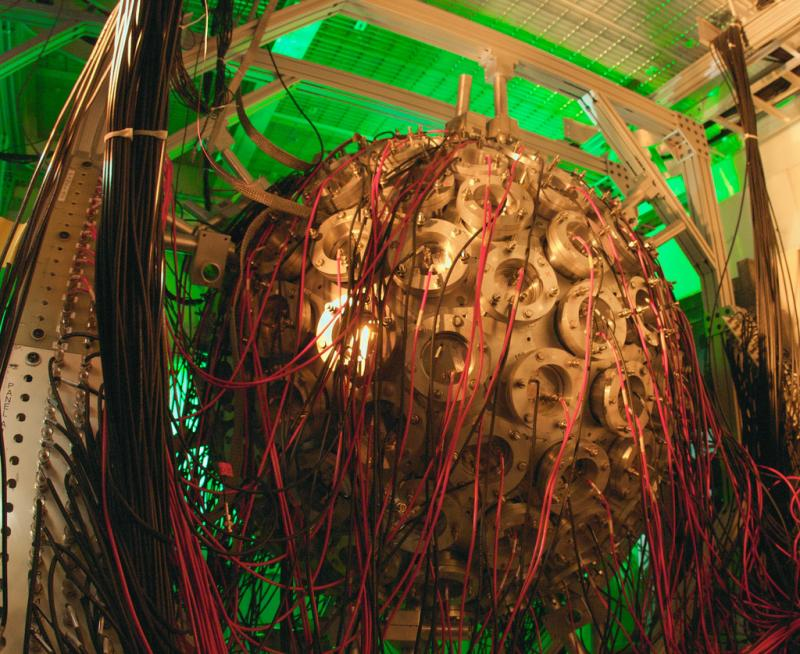
\includegraphics[scale=0.3]{dance1}
\end{frame}

\begin{frame}{DANCE}
\centering
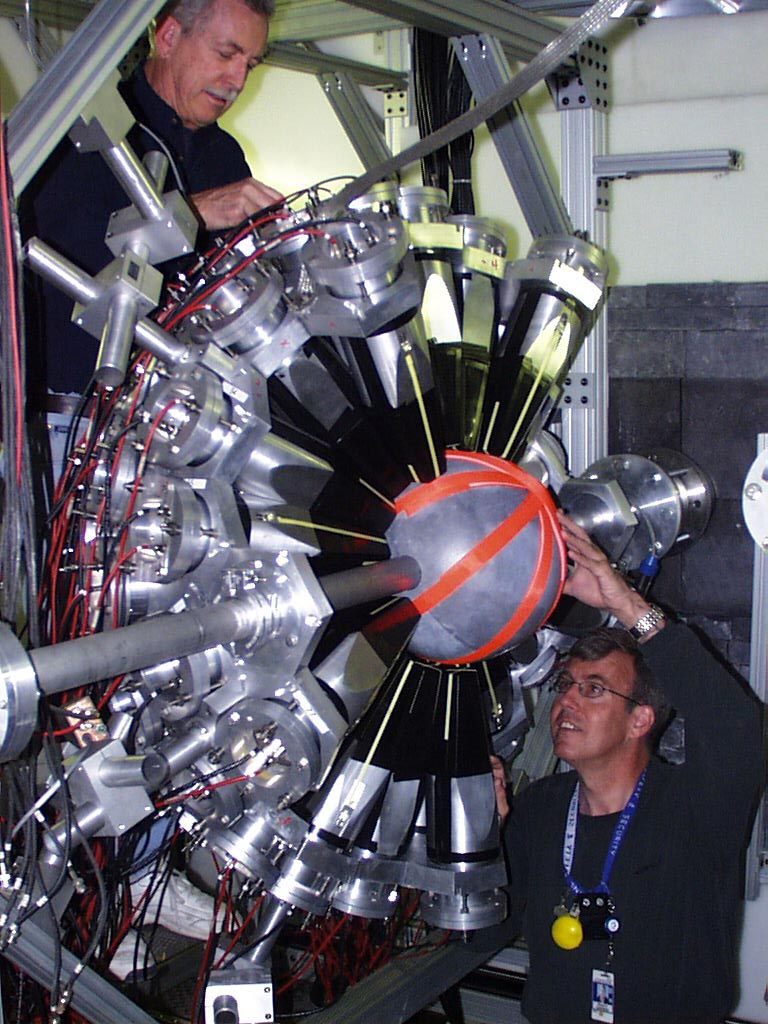
\includegraphics[scale=0.4]{dance2}
\end{frame}

\begin{frame}{NEUANCE}
\begin{columns}
  \begin{column}{0.65\textwidth}
    \begin{itemize}
    \item \textbf{NEU}tron detector \textbf{A}rray at DA\textbf{NCE}
    \item Designed to fit inside DANCE
    \item Will study capture cross section of isomeric states of actinides
    \item EJ-309 and stilbene were tested in earlier prototypes
    \item Stilbene was chosen due to higher light-output and better PSD performance
    \end{itemize}
  \end{column}
  \begin{column}{0.40\textwidth}
	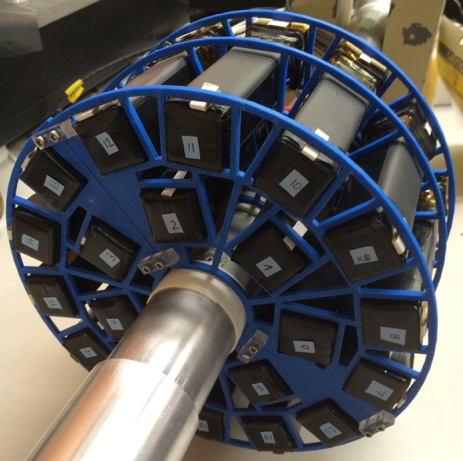
\includegraphics[scale = 0.25]{NeuancePicture}
  \end{column}
\end{columns}
\end{frame}


\subsection{Stilbene Detector}
\begin{frame}{Stilbene Detector}
\begin{itemize}
\item Organic scintillator
\item Higher light output and better PSD performance than EJ-309
\item NEUANCE detector array will incorporate 21 stilbene crystals
\item Approximate size: 2.3 cm x 2.3 cm x 10 cm
\item Each crystal will be coupled to a compact photomultiplier tube
\item Current efforts include improving modeling accuracy of a single stilbene crystal
\end{itemize}
\end{frame}

\begin{frame}{Photon Interactions in Stilbene}
\centering
\vskip -0.25cm
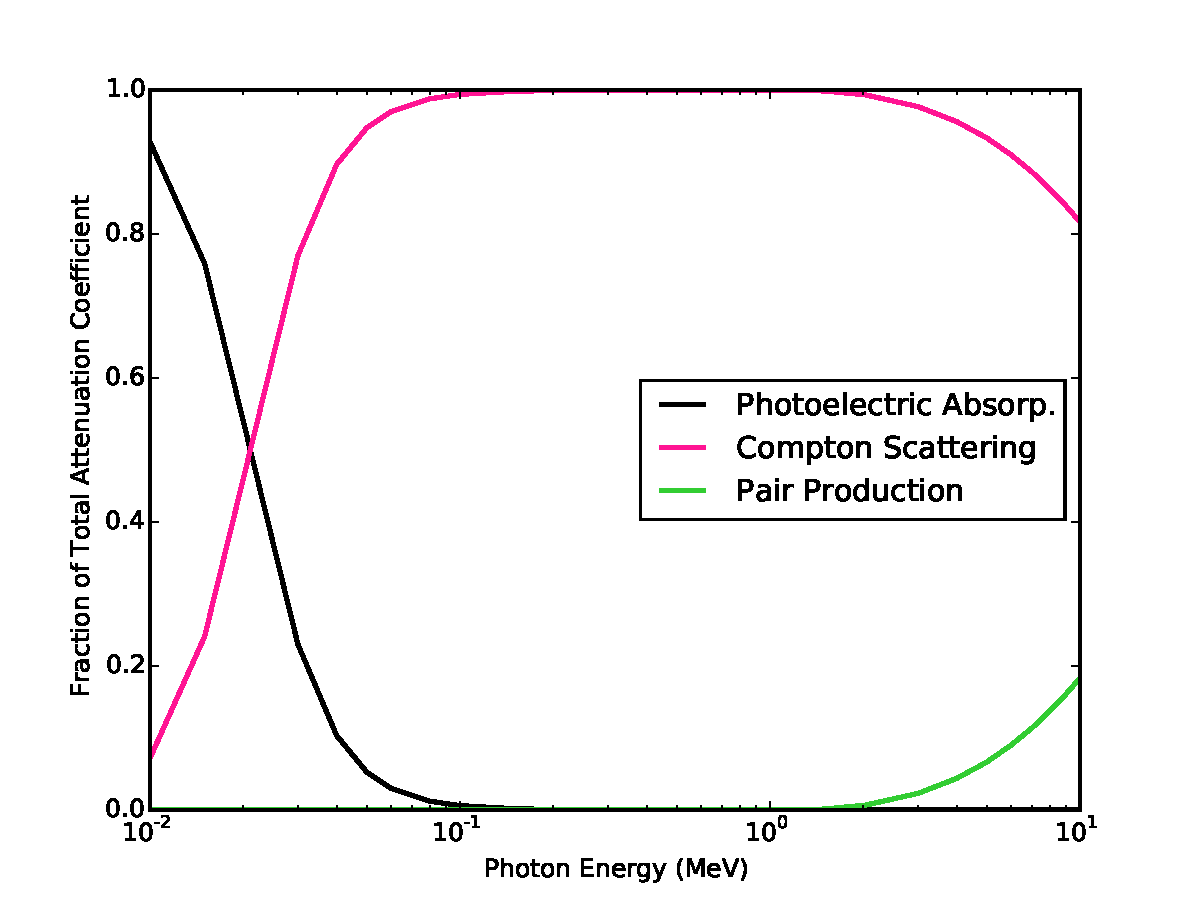
\includegraphics[scale=0.45]{interactionCoeff}
\end{frame}


\section{MCNP6 Settings}
\begin{frame}
\sectionpage
\end{frame}

\begin{frame}{MCNP6 Settings}
\begin{itemize}
\item Gaussian Energy Broadening (GEB)
  \begin{itemize}
  \item Virtual peak-broadening technique
  \item Converts gamma pulse height tally to approximate detector response function
  \item No parameters available for stilbene
  \end{itemize}
\item DE/DF
  \begin{itemize}
  \item Converts energy deposited by recoiled protons to electron equivalent energy
  \item Equation found in (Hansen, 2002)\cite{Hansen}
  \end{itemize}
\end{itemize}
\end{frame}

\subsection{GEB Parameters}
\begin{frame}{GEB Parameters - Iterative Method [Kim, 2015]}
  \begin{itemize}
  \item Calculate Compton edge for each peak
  \end{itemize}
  \begin{equation} \label{compton_edge}
  E_c = E_{e-}\vert_{(\theta=\pi)} = E_\gamma \left(\frac{2E_\gamma}{m_ec^2+2E_\gamma}\right)
  \end{equation}
  \begin{block}{Compton edges for gamma-ray sources:}
    \begin{center}
  \vskip -0.2cm
  \begin{tabular}{l  c  c}\toprule
   Element  & $E_\gamma$ (keV) & Compton Edge (keV) \\ \midrule \vspace{0.1cm}
   $^{133}$Ba & 356 & 207.25 \\
   $^{137}$Cs & 662 & 477.65 \\
   $^{54}$Mn & 835 & 639.36 \\
   $^{22}$Na (P.P.) & 511 & 340.67 \\
   $^{60}$Co & 1173 & 963.42 \\
   $^{22}$Na & 1274 & 1061.18 \\
   $^{60}$Co & 1332 & 1118.10 \\ \bottomrule
  \end{tabular}
  \end{center}
  \end{block}
\end{frame}

\begin{frame}{GEB Parameter - Iterative Method [Baramsai, 2015]}
\begin{itemize}
\item Calibrate spectra using Compton edge as Compton maximum
\end{itemize}
\begin{figure}
\vspace*{-0.3cm}
\begin{center}
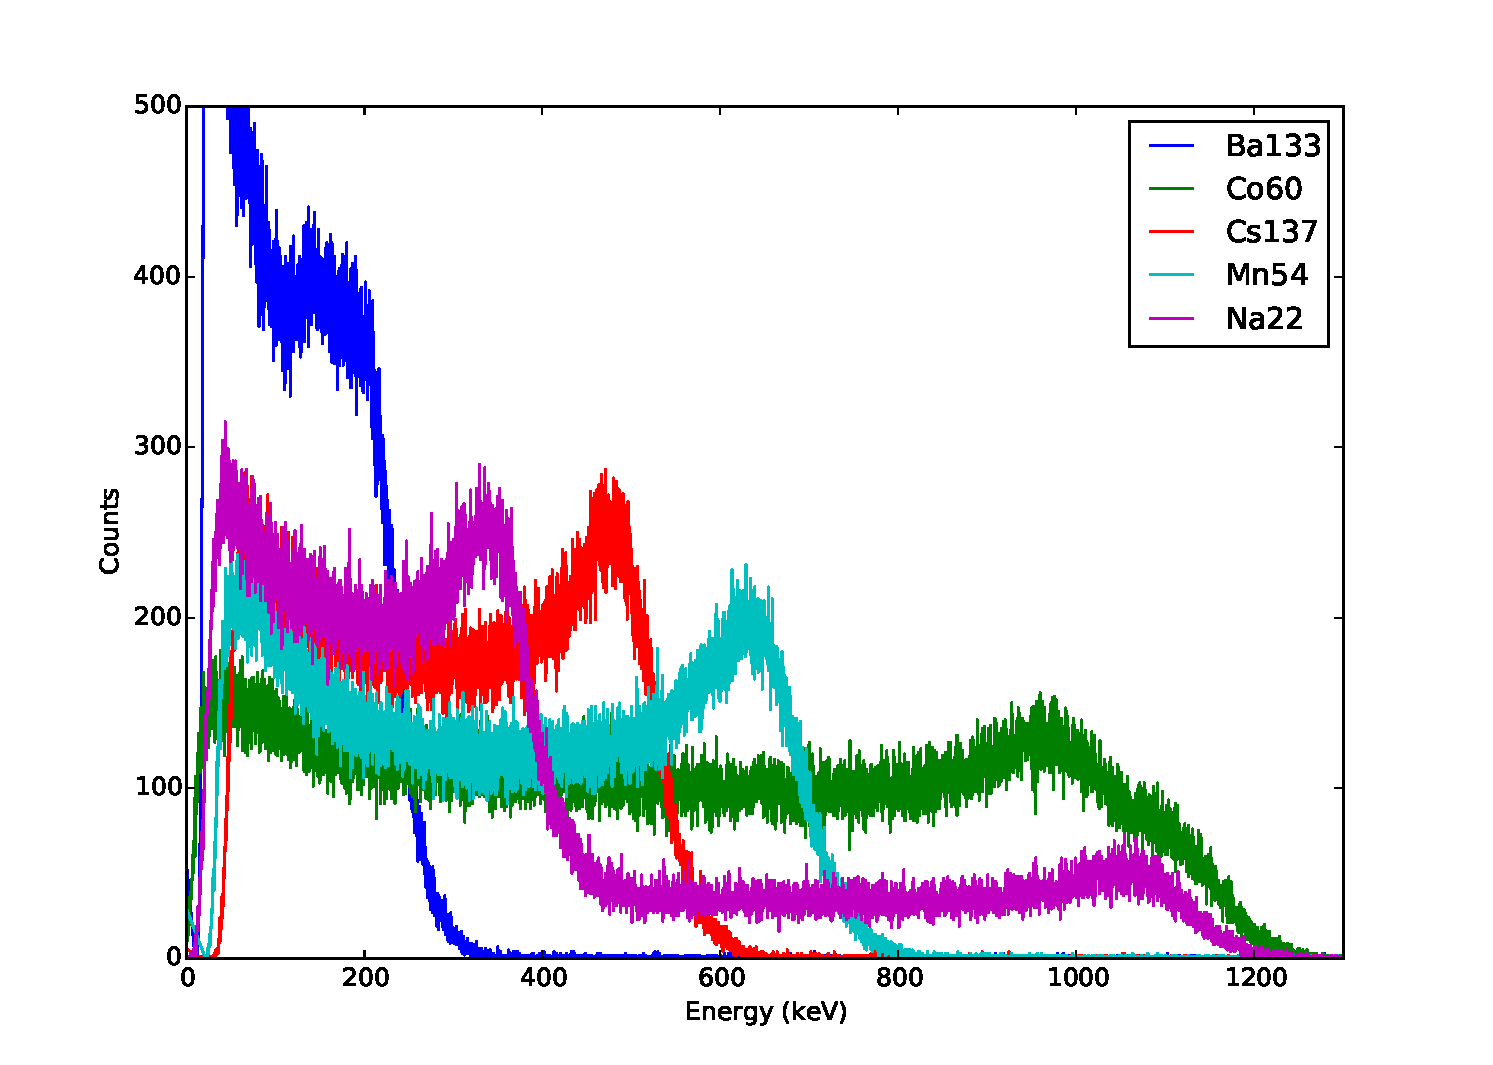
\includegraphics[scale = 0.28]{1stCalibration}
\caption{\scriptsize{First Calibration, Assumption: Compton Edge = Compton Maximum}}
\end{center}
\end{figure}
\end{frame}


\begin{frame}{GEB Parameters - Iterative Method [Kim, 2015]}
  \begin{columns}
      \begin{column}{0.5\textwidth}
		\begin{itemize}
        \item Fit Gaussian function to experimental data using equation \ref{peak_fit}. \cite{Kim}
        \end{itemize}
        \begin{equation} \label{peak_fit}
          f(E) = C e^{-\frac{2\sqrt{\ln{2}}(E - E_0)}{FWHM}^2}
        \end{equation}
        \begin{itemize}
        \item Set $E_0$ = Compton maxima 
		\item Fit function to obtain constant (C) and FWHM
		\end{itemize}
	\end{column}
	\begin{column}{0.5\textwidth}
	   \begin{figure}[H]
       \vspace*{-1cm}
       \begin{center}
	   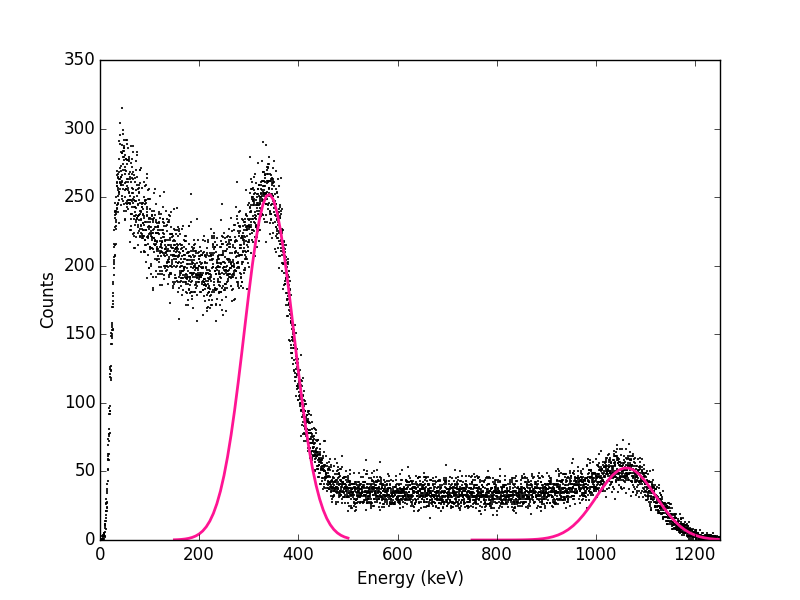
\includegraphics[scale = 0.3]{GaussPeakFit}
       \caption{\scriptsize{$^{22}$Na Gaussian Peak Fit}}
	   \end{center}
      \end{figure}
	\end{column}
  \end{columns}
\end{frame}

\begin{frame}{GEB Parameters - Iterative Method [Kim, 2015]}
  \begin{itemize}
  \item Use FWHM from Eq. \ref{peak_fit} to find fitting parameters (a, b, c)
  \end{itemize}
  \begin{equation} \label{FWHM}
  FWHM(E_o) = a + b \sqrt{E_o + c E_o^2}
  \end{equation}
\vspace{-0.5cm}
  \begin{columns}
    \begin{column}{0.3\textwidth}
      \begin{block}{After 1$^{st}$ iteration:}
      \begin{itemize}
      \item a = -0.049702
      \item b =  0.267462
      \item c = -0.526174
      \end{itemize}
      \end{block}
	\end{column}
	\begin{column}{0.5\textwidth}
      \begin{figure}
      \begin{center}
      \vspace{-0.5cm}
      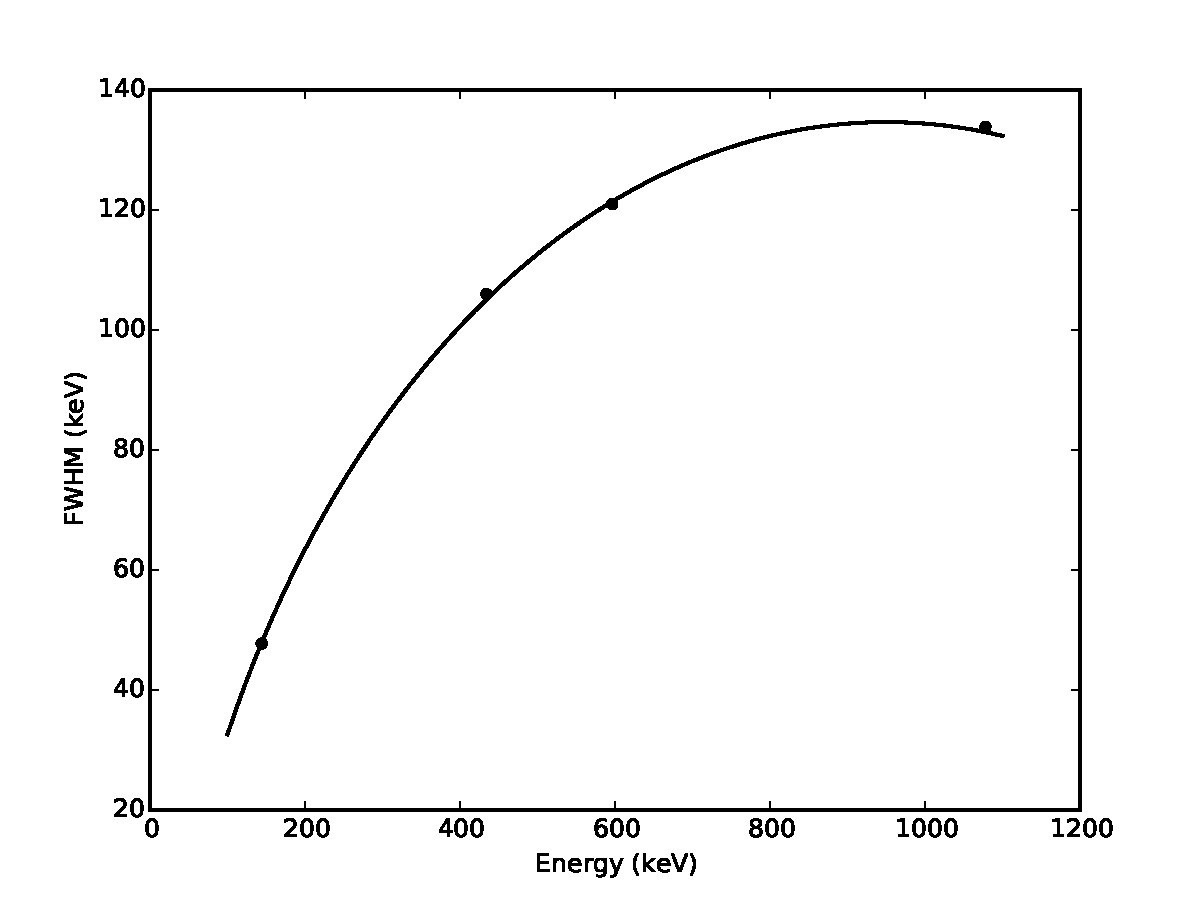
\includegraphics[scale=0.3]{FWHM_values1}
      \vspace{-0.5cm}
      \caption{\scriptsize{FWHM Curve for Stilbene}}
      \end{center}
      \end{figure}
	\end{column}
  \end{columns}
\end{frame}

\begin{frame}{GEB Parameters - Iterative Method}
\begin{figure}
\vspace{-0.25cm}
\begin{center}
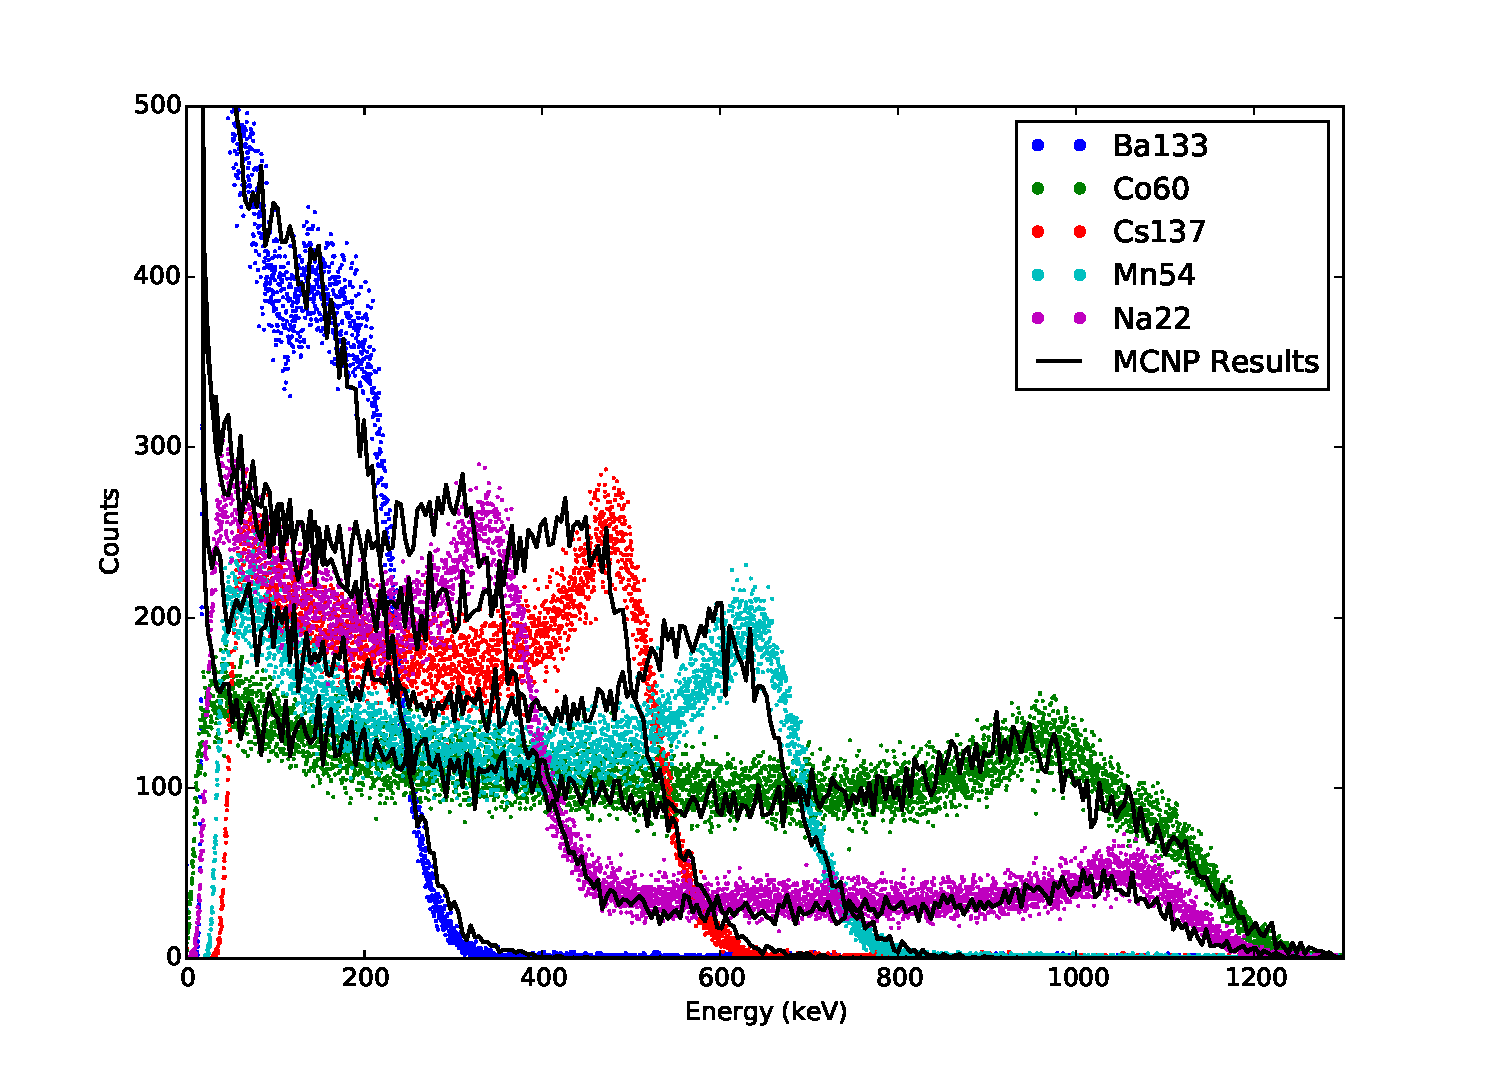
\includegraphics[scale = 0.35]{MCNP_Comparison_1cal}
\vspace{-0.4cm}
\caption{\scriptsize{1$^{st}$ MCNP Iteration}}
\end{center}
\end{figure}
\end{frame}

\begin{frame}{GEB Parameters - Iterative Method [Kim, 2015]}
  \begin{itemize}
  \item Re-calibrate spectra using Compton maxima from MCNP
  \item Fit Gaussian functions to each peak
  \end{itemize}
\vspace*{-0.5cm}
  \begin{columns}
    \begin{column}{0.4\textwidth}
    \vspace*{-0.2cm}
	\begin{itemize}
    \item Fit parameters:
    \end{itemize}
    \vspace*{0.3cm}
 	\[\small{FWHM(E_o) = a + b \sqrt{E_o + c E_o^2}}\]
      \begin{block}{After 2$^{nd}$ iteration:}
  	  \begin{itemize}
      \item a = -0.057192
      \item b =  0.249732
      \item c = -0.432120
      \end{itemize}
	\end{block} 
	\end{column}
	\begin{column}{0.5\textwidth}
      \begin{figure}
      \begin{center}
      \vspace{-0.5cm}
      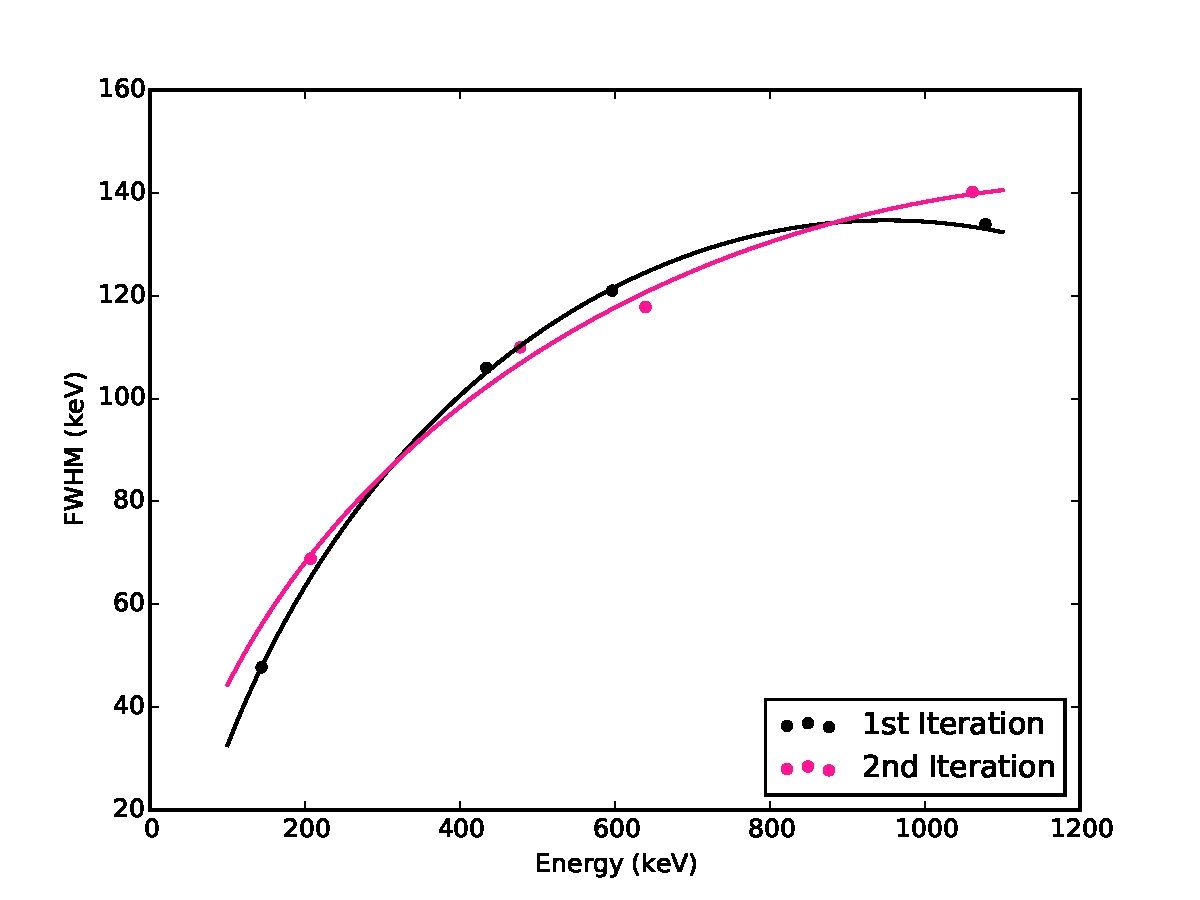
\includegraphics[scale=0.3]{FWHM_values2}
      \vspace{-0.5cm}
      \caption{\scriptsize{FWHM Curves for Stilbene}}
      \end{center}
      \end{figure}
	\end{column}
  \end{columns}
\end{frame}


\begin{frame}{GEB Parameters - Iterative Method}
\begin{figure}
\vspace{-0.25cm}
\begin{center}
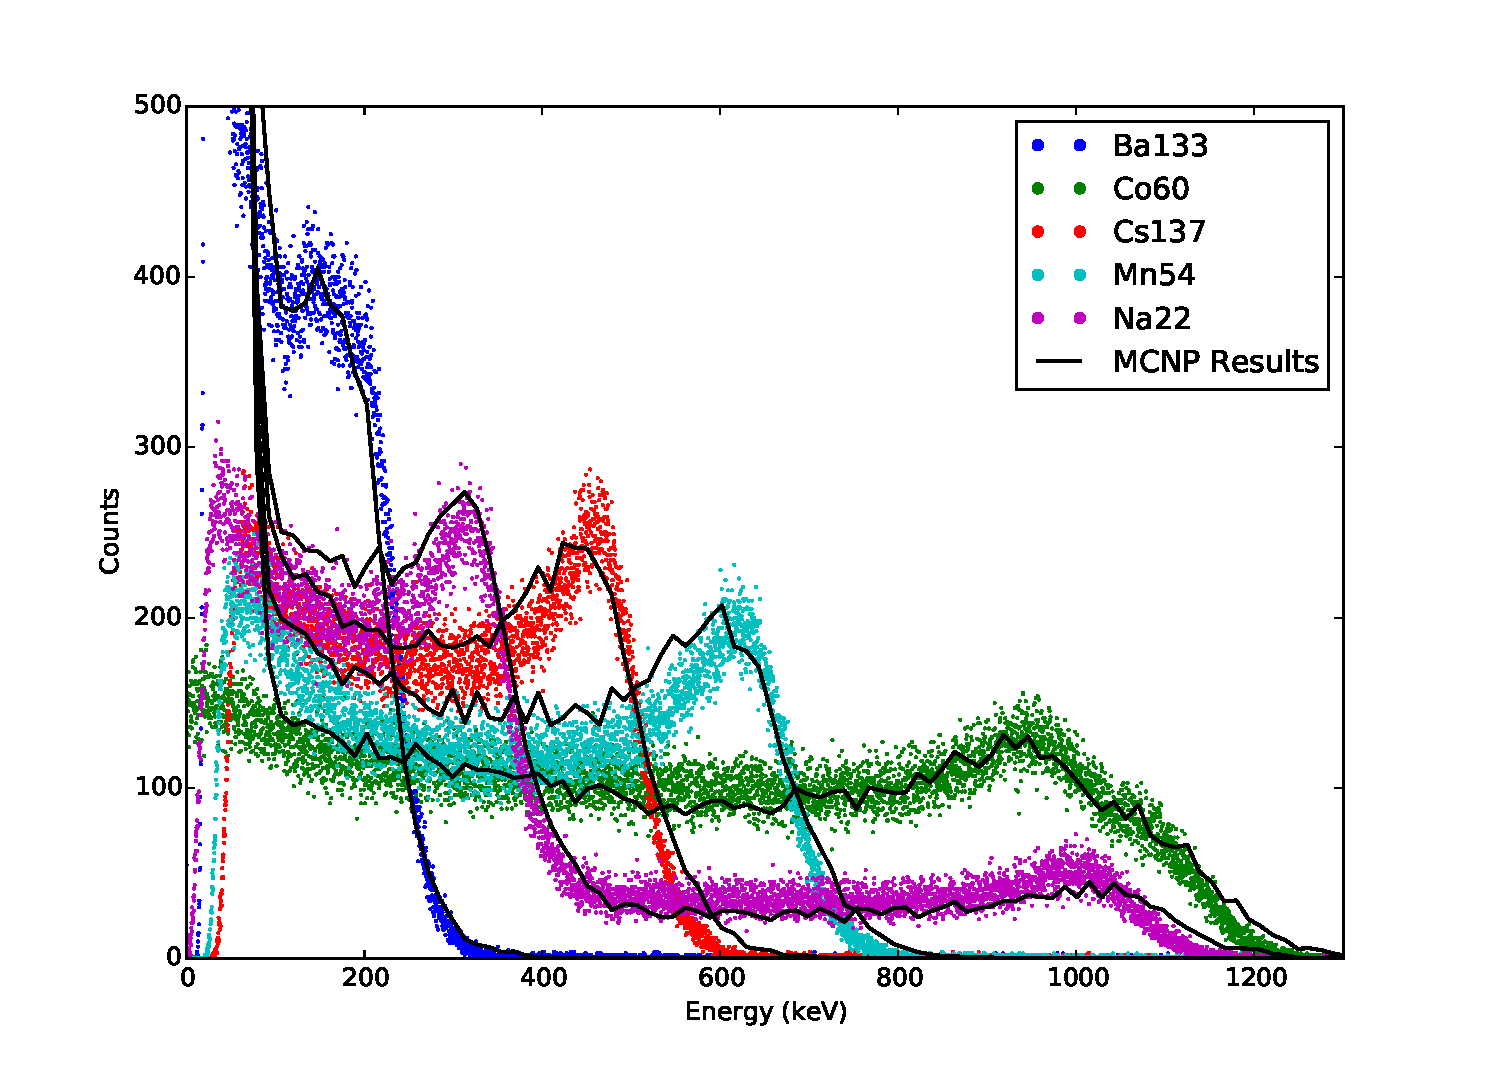
\includegraphics[scale = 0.35]{MCNP_Comparison_2cal}
\vspace{-0.4cm}
\caption{\scriptsize{2$^{nd}$ MCNP Iteration}}
\end{center}
\end{figure}
\end{frame}

\subsection{DE and DF Cards}
\begin{frame}{DE and DF Cards [Hansen, 2002]}
\vspace*{-0.3cm}
\begin{itemize}
\item Non-linear light output function for stilbene:
\end{itemize}
  \begin{equation} \label{Light_output}
  L = aE_p - b[1-exp(-cE_p^d)]
  \end{equation}
 \vspace*{-0.3cm}
\begin{itemize}
\item Converts recoil proton energy ($E_p$), to light output due to energy deposited by the effective electron equivalent energy ($L$)
\end{itemize}
\begin{block}{Optimization constants found in [Hansen, 2002]:}
\begin{itemize}
\item a=0.693
\item b=3.0
\item c= 0.2
\item d=0.965
\end{itemize}
\end{block}
\end{frame}

\begin{frame}{Simulation Results: \textsuperscript{252}Cf}
\vspace*{-0.4cm}
\begin{figure}
\begin{center}
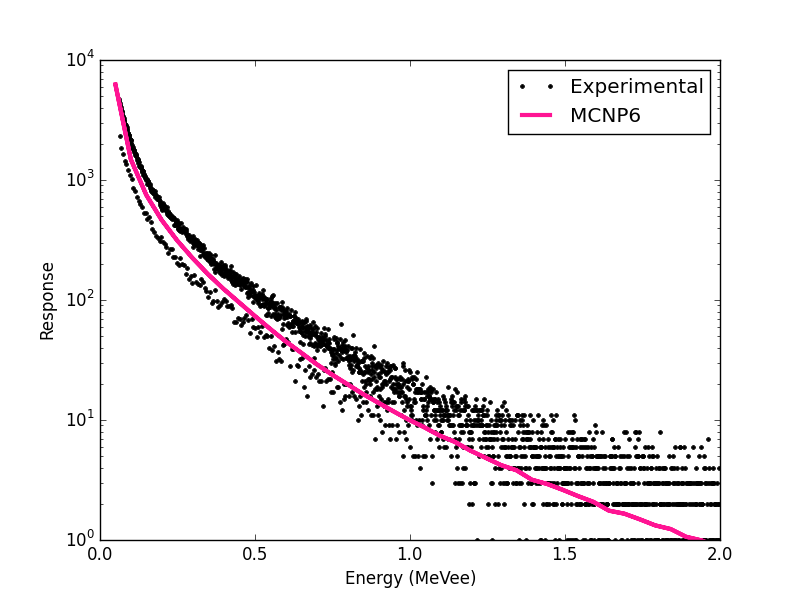
\includegraphics[scale = 0.41]{Cf252}
\vspace*{-0.4cm}
\caption{\scriptsize{MCNP6 vs Experimental measurements using the DE/DF tally treatment}}
\end{center}
\end{figure}
\end{frame}

\section{DRiFT}
\begin{frame}
\sectionpage
\end{frame}

\begin{frame}{DRiFT}
\vskip-2.2cm
\begin{itemize}
\item Stilbene processing capabilities have been added to DRiFT
  \begin{itemize}
  \item Light output function (Equation \ref{Light_output})
  \item Light emission spectrum (Left)
  \item Neutron and gamma pulse shapes - in progress (Center)
  \item PMT Quantum Efficiency(Right)
  \end{itemize}
\end{itemize}
%%% Left
\begin{tikzpicture}[remember picture, overlay]
\node [xshift = -10.7cm, yshift=2.4cm] at (current page.south east){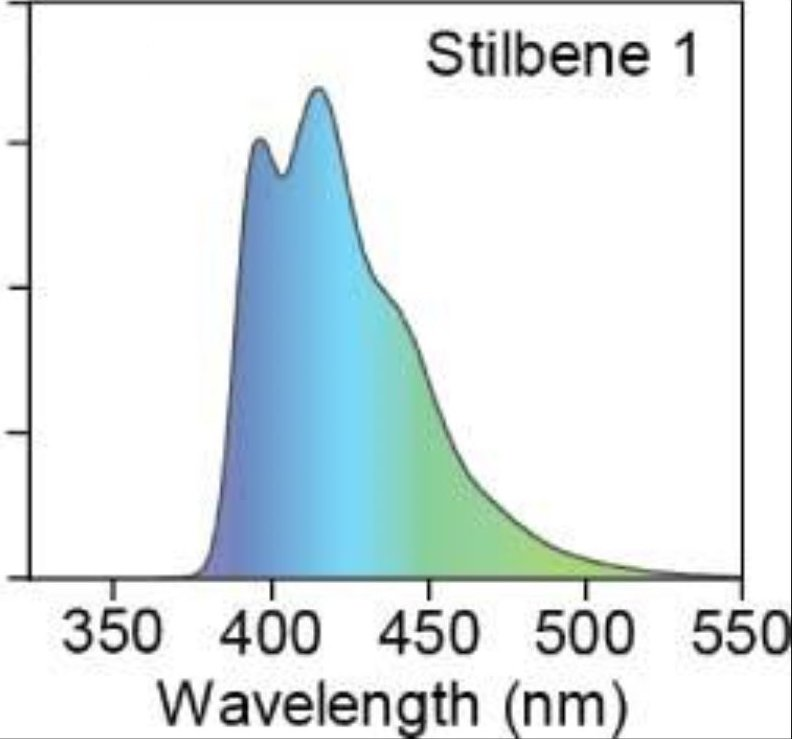
\includegraphics[scale=0.16]{Emission_Spectrum}};
\end{tikzpicture}
%%% Center
\begin{tikzpicture}[remember picture, overlay]
\node [xshift = -6.3cm, yshift=2.5cm] at (current page.south east){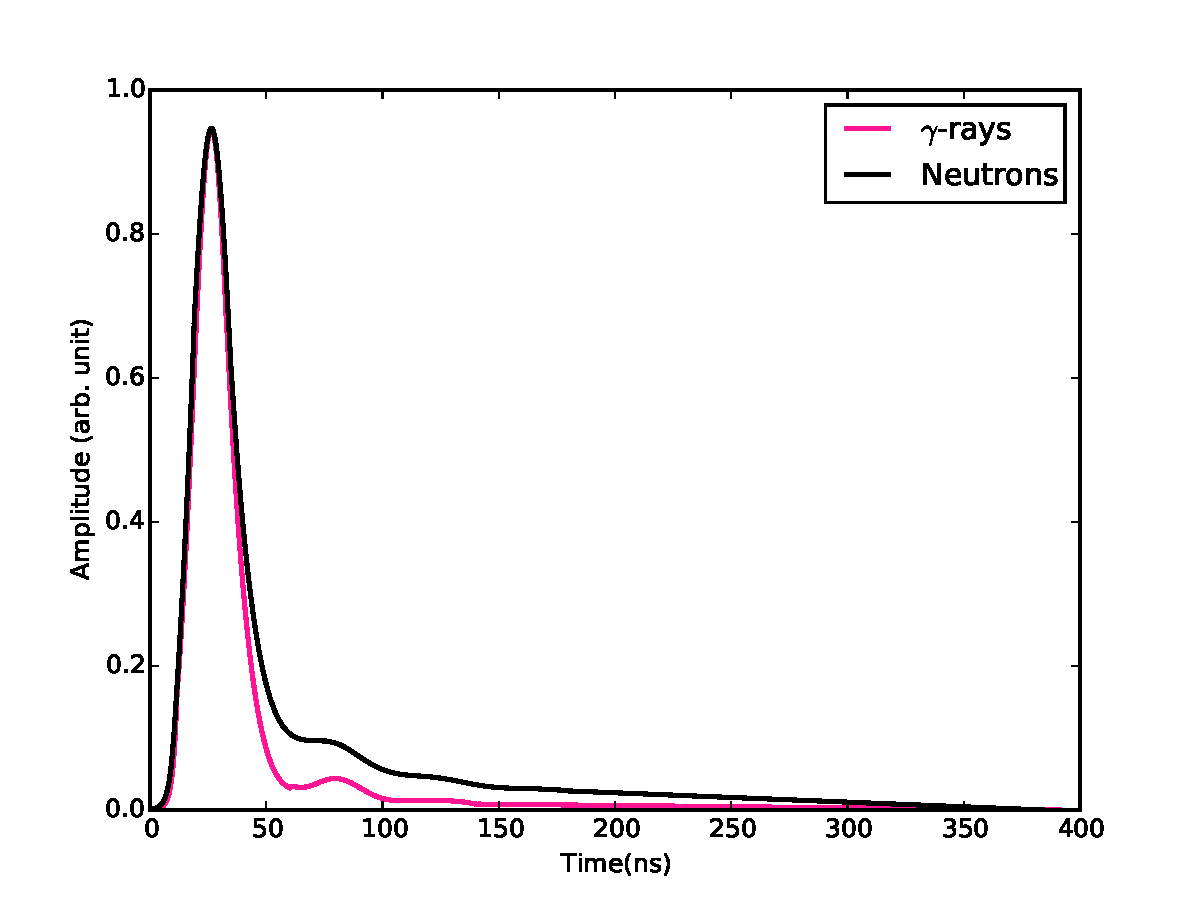
\includegraphics[scale=0.24]{Stilbene_PSD}};
\end{tikzpicture}
%%% Right
\begin{tikzpicture}[remember picture, overlay]
\node [xshift = -2.1cm, yshift=2.5cm] at (current page.south east){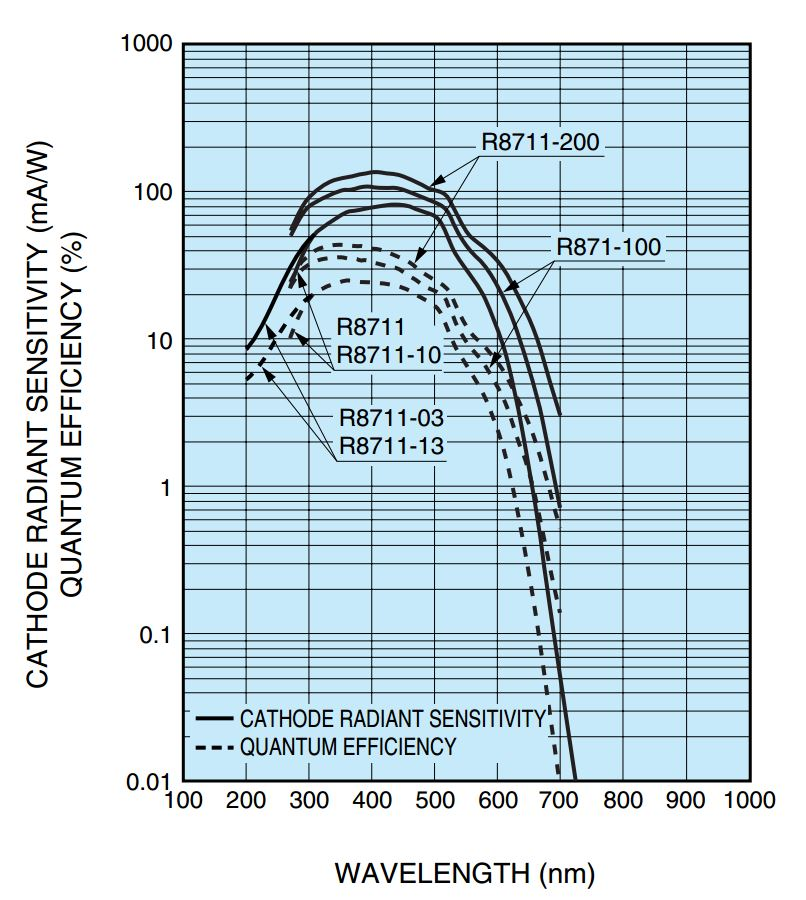
\includegraphics[scale=0.18]{Hamamatsu_R87_series}};
\end{tikzpicture}
\end{frame}

\begin{frame}{Preliminary DRiFT Results: Gamma Rays}
\vspace*{-0.3cm}
\begin{figure}
\begin{center}
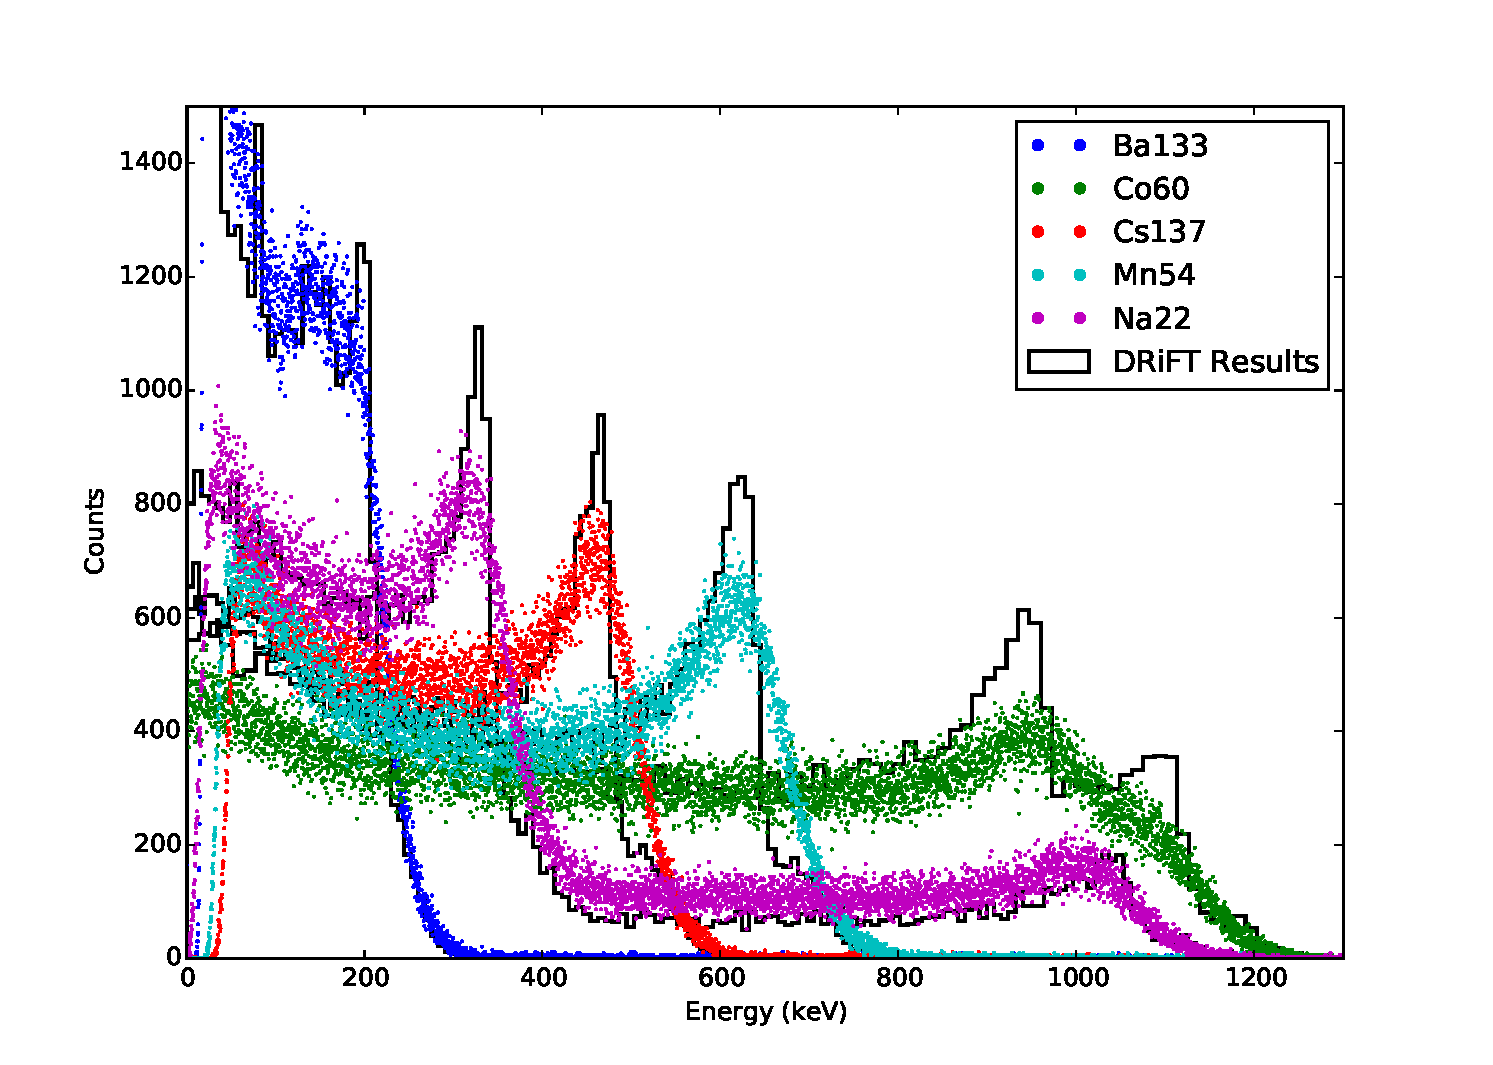
\includegraphics[scale = 0.38]{DRiFT_Comparison}
\vspace*{-0.5cm}
\caption{\scriptsize{DRiFT vs Experimental gamma-ray measurements}}
\end{center}
\end{figure}
\end{frame}

\begin{frame}{Preliminary DRiFT Results - Neutrons}
\vspace*{-0.3cm}
\begin{figure}
\begin{center}
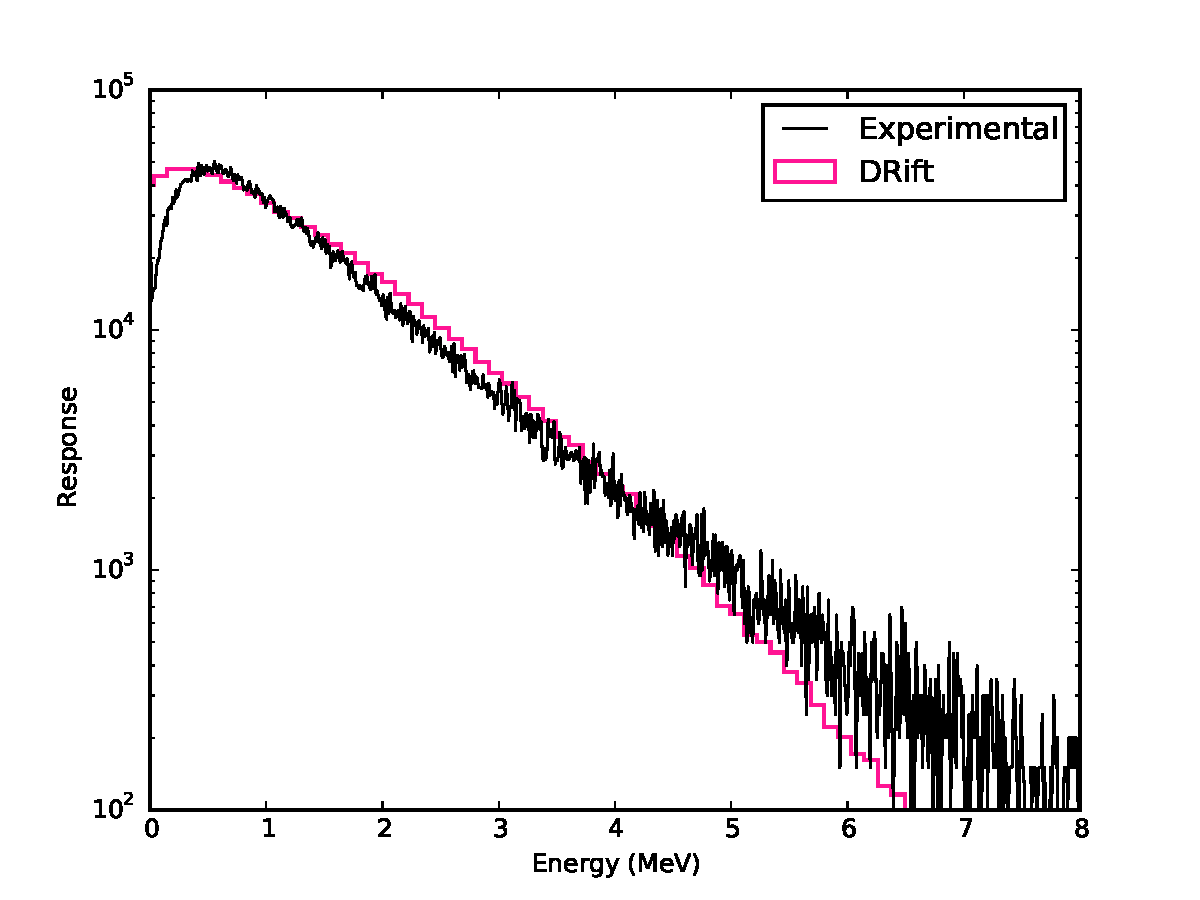
\includegraphics[scale = 0.45]{drift_neutrons}
\vspace*{-0.5cm}
\caption{\scriptsize{DRiFT vs Experimental \textsuperscript{252}Cf measurements}}
\end{center}
\end{figure}
\end{frame}

\section{Future Work}
\begin{frame}
\sectionpage
\end{frame}

\begin{frame}{Future Work}
\begin{itemize}
\item Continue improving stilbene modeling parameters and capabilities in DRiFT
\begin{itemize}
\item PSD using waveforms
\item Low-energy photon detection improvements 
\end{itemize}2
\item Begin modeling multiple stilbene detectors in different angle configurations
\item Model full NEUANCE detector array
\item Study detector cross-talk
\item Compare MCNP6/DRiFT simulations using CGMF/FREYA against experimental measurements
\begin{itemize}
\item \textsuperscript{252}Cf: spontaneous fission
\item \textsuperscript{239}Pu and \textsuperscript{235}U: neutron-induced fission
\end{itemize}
\end{itemize}
\end{frame}

\appendix
\section{Questions?}
\begin{frame}
\sectionpage
\end{frame}

\begin{frame}[allowframebreaks]{References}
\def\newblock{}
\nocite{*}
\scriptsize{\bibliographystyle{plain}}
\bibliography{references}
\end{frame}

\end{document}
